\section{Nezávislé jevy}

Klíčovým pojmem v teorii pravděpodobnosti jsou tzv. \emph{nezávislé jevy}. Nejprve si uveďme definici a následně se podíváme na několik příkladů.

\begin{definition}[Nezávislé jevy]\label{def:nezavisle_jevy}
    Libovolné jevy $A,\,B\subseteq\Omega$ nazýváme \textbf{nezávislé}, pokud platí
    \[\Prob(A\cap B)=\Prob(A)\cdot\Prob(B).\]
    V opačném případě nazveme nazveme jevy $A,\,B$ \textbf{závislými}.
\end{definition}

Tuto definici můžeme zobecnit na libovolný počet jevů, tj. jevy $A_1,\,A_2,\,\dots,\,A_n\subseteq\Omega$ nezveme nezávislými, pokud platí
\[\Prob\left(\bigcap\limits_{i=1}^{n}A_i\right)=\prod_{i=1}^{n}\Prob(A_i).\]
\medskip

Tato definice se může zdát poměrně abstraktní. Avšak název reflektuje poměrně jednoduchou věc a to sice, že jsou-li jevy $A,\,B$ nezávislé, pak tvrdíme, že výskyt jevu $A$ \textbf{nijak neovlivní výskyt} $B$. Často se této vlastnosti využívá, pokud chceme vypočítat pravděpodobnost, že nastane jev $A$ a zároveň i jev $B$, tzn. jev $A\cap B$.\par
J. Nešetřil ve své knize \emph{Kapitoly z diskrétní matematiky} vysvětluje nezávislost jevů následovně: \textit{Nezávislost znamená, že rozdělíme-li $\Omega$ na dvě části, jev $A$ a jeho doplněk $\Omega\setminus A$, pak jev $B$ "rozřízne" obě tyto části v témže poměru. Jinak řečeno, kdybychom prvek $\omega\in\Omega$ volili náhodně nikoliv ze všech prvků $\Omega$, ale jenom mezi prvky $A$, byla by pravděpodobnost, že $\omega\in B$, přesně rovna $\Prob(B)$ (za předpokladu, že $\Prob(A)\neq 0$).} \citep[str. 314]{MatousekNesetril2009}
\begin{figure}[H]
    \centering
    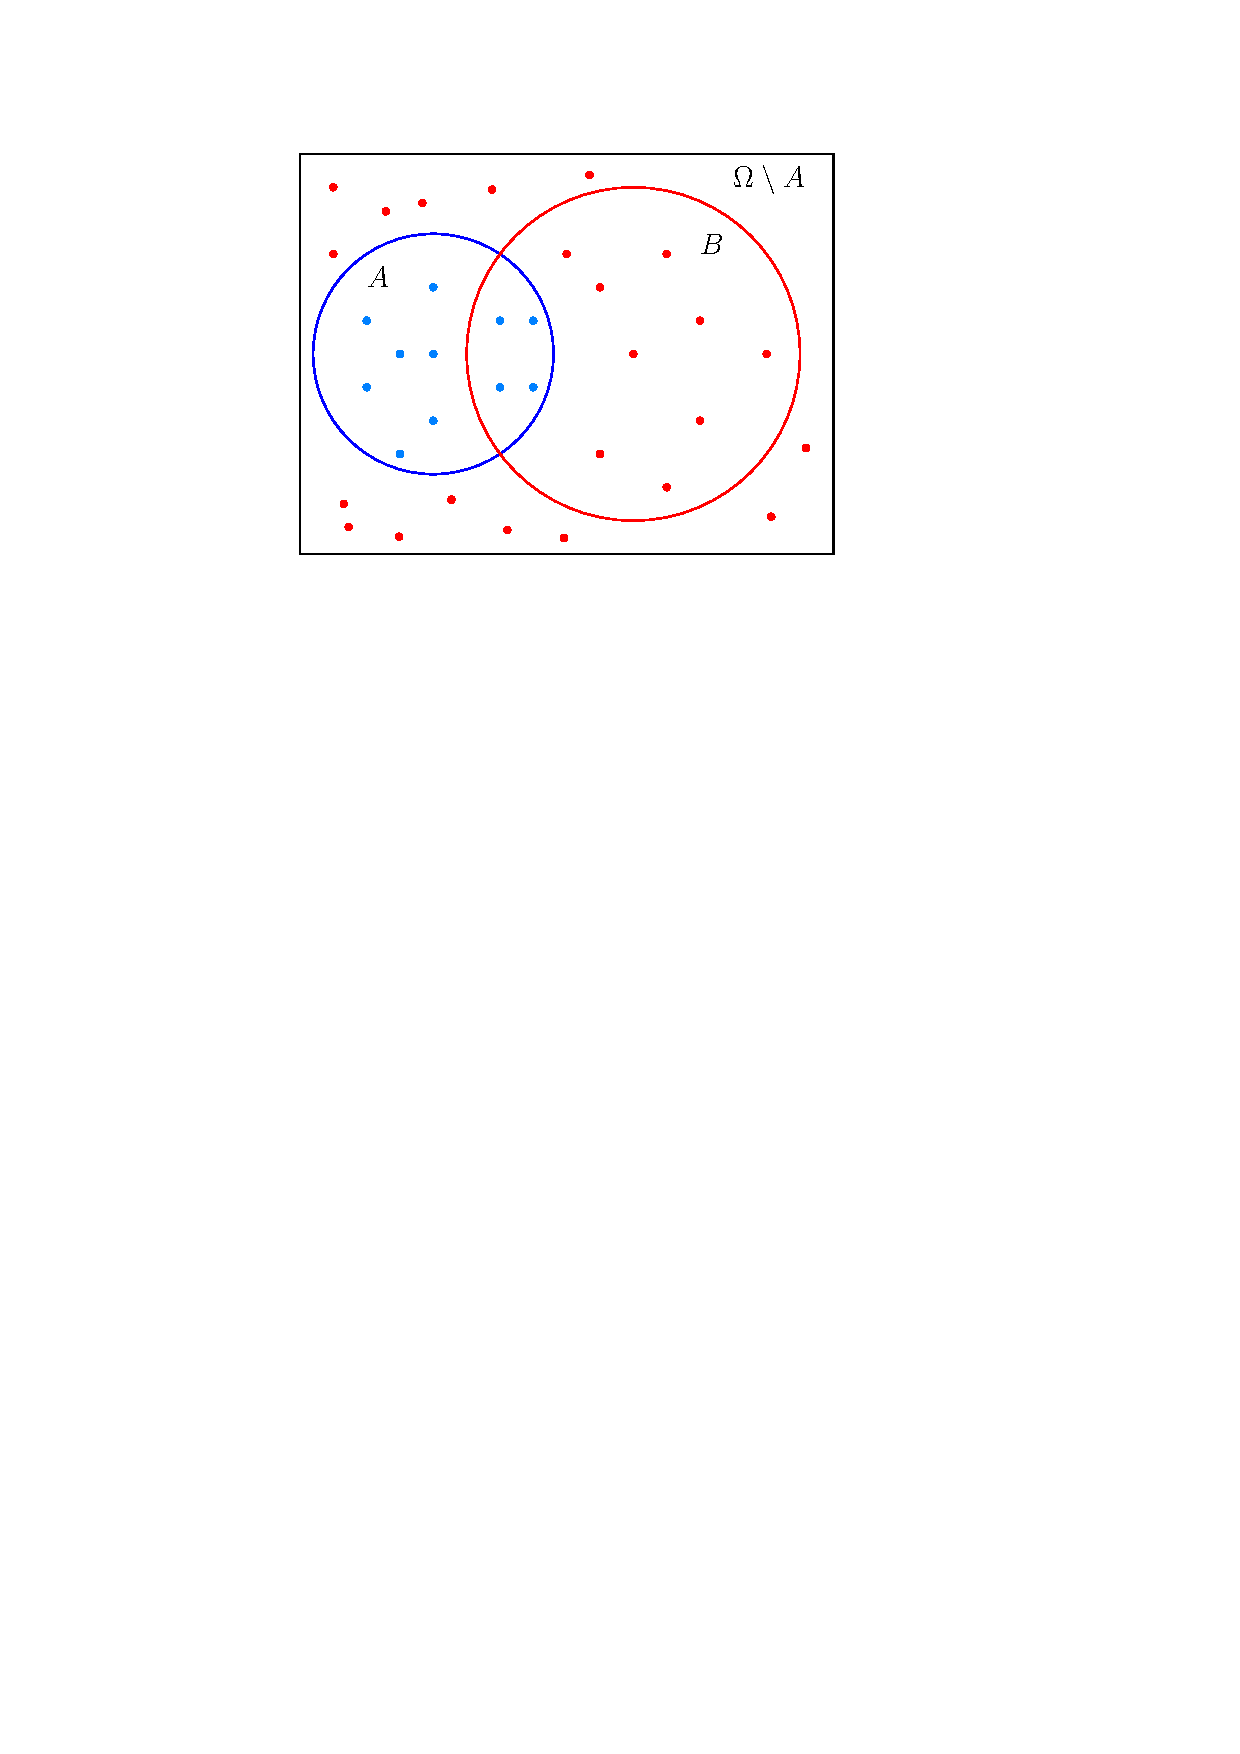
\includegraphics[scale=\normalipe]{ch04_nezavislost_jevu.pdf}
    \caption{Grafické znázornění nezávislosti jevů.}
    \label{fig:nezavislost_jevu}
\end{figure}
Na obrázku \ref{fig:nezavislost_jevu} lze vidět grafické znázornění k vysvětlení výše. Poměr počtu červeně vyznačených elementárních jevů, které náleží jevu $B$ a počtu elementárních jevů, které mu nenáleží, ale náleží $\Omega\setminus A$, je stejný, jako poměr počtu elementárních jevů, které náleží $A$, ale nikoliv $B$, a počtu elementárních jevů, které náleží $A\cap B$. Protože všechny elementární jevy jsou stejně pravděpodobné, pak příslušné poměry přímo odpovídají daným pravděpodobnostem. tzn.
\[\dfrac{\sizeof{A\cap B}}{\sizeof{A}}=\dfrac{\sizeof{B\setminus A}}{\sizeof{\Omega\setminus A}}\]
\begin{task}
    Házíme $n$-krát spravedlivou mincí. Jaká pravděpodobnost, že 2-krát za sebou padne líc?
\end{task}
\begin{solution}
    První hod mince jistě nijak neovlivní druhý hod. Protože házíme dvakrát, množinu elementárních jevů nyní tvoří uspořádané dvojice, kdy první, resp. druhá souřadnice značí, zda v prvním, resp. druhém hodu padl rub (R) nebo líc (L), tj. $\Omega=\set{(R,\,R),\,(R,\,L),\,(L,\,R),\,(L,\,L)}$. Jev, kdy v prvním hodu padl líc, si označíme $A=\set{(L,\,R),\,(L,\,L)}$, a jev, kdy padl v druhém hodu líc, si označíme $B=\set{(R,\,L),\,(L,\,L)}$. Protože nás zajímá, kdy padne v obou hodech líc, pak nás zajímá jev $A\cap B=\set{(L,\,L)}$. Tedy pravděpodobnost, že tento jev nastane, je
    \[\Prob(A\cap B)=\dfrac{\sizeof{A\cap B}}{\sizeof{\Omega}}=\dfrac{1}{4}=25\,\%.\]
    Avšak, jak se můžeme přesvědčit, platí také
    \[\Prob(A\cap B)=\Prob(A)\cdot\Prob(B)=\dfrac{1}{2}\cdot\dfrac{1}{2}=\dfrac{1}{4}.\]
    Jevy $A$ a $B$ jsou tedy \textbf{nezávislé}.
\end{solution}
Jedna věc se zde může zdát zarážející. Pokud se ohlédneme zpět za definicí nezávislých jevů \ref{def:nezavisle_jevy}, můžeme si všimnout, že ačkoliv nám definice dává v podstatě "návod", jak počítat pravděpodobnost nezávislých jevů, přesto jsme se u příkladu výše byly "nuceni" uchýlit ke klasickému výpočtu pravděpodobnosti z definice, tj. \emph{počet příznivých možností ke počtu všech možných možností}, a to proto, že jsme dopředu nevěděli, zda uvažované jevy jsou skutečně nezávislé a museli jsme tuto skutečnost ověřit výpočtem. Nezdá se, že tak naše definice byla něčemu užitečná. Ale není tomu tak, neboť si stačí uvědomit následující věc. Představme si, že máme množinu elementárních jevů $\Omega=\set{\omega_1,\,\omega_2,\,\dots,\,\omega_n}$ a libovolné disjunktní jevy $A,\,B\subseteq\Omega$. Uvažme, že chceme vypočítat pravděpodobnost, že při dvou pokusech nejdříve nastane jev $A$ a pak jev $B$. Pak tuto pravděpodobnost lze stanovit právě pomocí vzorce
\[\Prob(A\cap B)=\Prob(A)\cdot\Prob(B).\]
Je tomu tak z důvodu, že pokud provádíme dva pokusy, pak množina všech možných jevů, označme $\Omega^\prime$, obsahuje uspořádané dvojice (jako u úlohy s hodem mincí), tj. $\Omega^\prime=\set{(\omega_i,\,\omega_j)\admid 0\leqslant i,\,j\leqslant n}$ (tedy zde započítáváme i kolik pokusů provádíme; obecně pokud bychom prováděli $k$ pokusů, pak tato množiny bude obsahovat uspořádané $k$-tice). Tzn. jev $A\cap B$ obsahuje všechny dvojice, které náleží jak jevu $A$, tak jevu $B$, tj. takové, které na příslušných souřadnicích mají elementární jevy z $A$ a $B$. Formálně zapsáno:
\[A\cap B=\set{(\varphi,\,\psi)\admid\varphi\in A \land \psi\in B}.\]
Chceme nyní vypočítat $\Prob(A\cap B)$. K tomu potřebujeme znát $\sizeof{A\cap B}$ a $\sizeof{\Omega^\prime}$. Protože víme, že $\sizeof{\Omega}=n$ a $\Omega^\prime$ je množina všech uspořádaných dvojic z elementárních jevů $\Omega$, pak $\sizeof{\Omega^\prime}=n^2$.\par
Velikost průniku $A\cap B$ lze určit následující úvahou. Pokud elementární jevy jevu $A$ obsahují na první souřadnici elementární jevy množiny $\Omega$, které si označíme
\[\varphi_1,\,\varphi_2,\,\dots,\,\varphi_m,\]
pak $\sizeof{A}=mn$. Analogicky pro obsahující uspořádané dvojice, kde na druhé souřadnici jsou elementární jevy
\[\psi_1,\,\psi_2,\,\dots,\,\psi_k,\]
pak $\sizeof{B}=kn$. Tedy pravděpodobnost, že nastane jev $A$, je tak
\[\Prob(A)=\dfrac{\sizeof{A}}{\sizeof{\Omega}}=\dfrac{mn}{n^2}=\dfrac{m}{n}\]
a analogicky pro $B$ je pravděpodobnost
\[\Prob(B)=\dfrac{\sizeof{B}}{\sizeof{\Omega}}=\dfrac{kn}{n^2}=\dfrac{k}{n}.\]
Pravděpodobnosti těchto jevů tedy vyjadřují podíl daných jevů vůči všem možnostem.
\begin{figure}[H]
    \centering
    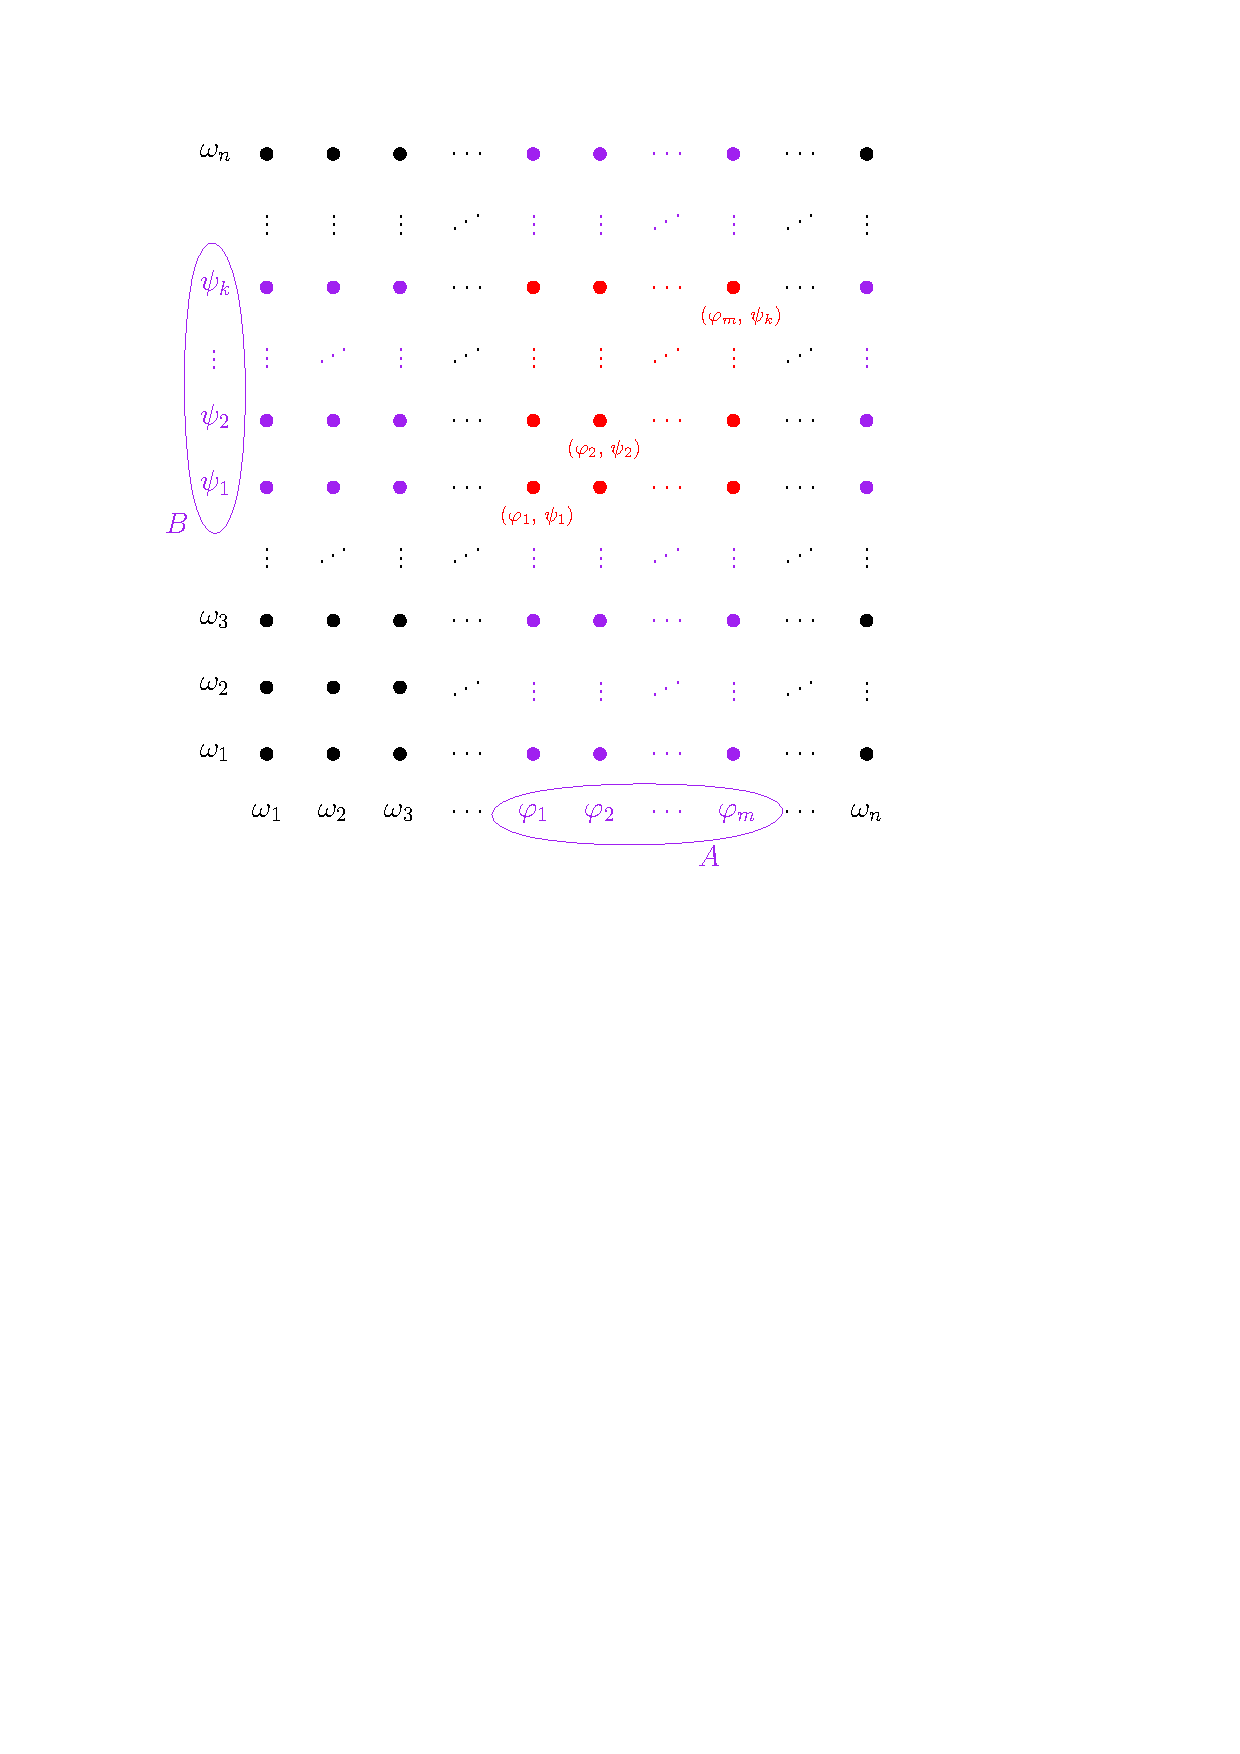
\includegraphics[scale=\normalipe]{ch04_dvojice_podil.pdf}
    \caption{Znázornění jevů $A$ a $B$ v množině $\Omega^\prime$.}
    \label{fig:dvojice_podil}
\end{figure}
Z obrázku si však můžeme uvědomit, že podíl počtu elementární jevů $A$ a všech elementárních jevů musí být stejný jako podíl počtu elementárních jevů jevu $A\cap B$ a počtu elementárních jevů jevu $B$. To znamená, že platí
\[\dfrac{\sizeof{A}}{\sizeof{\Omega^\prime}}=\dfrac{\sizeof{A\cap B}}{\sizeof{B}}.\]
Z této rovnosti již dokážeme vyjádřit $\sizeof{A\cap B}$, tj.
\[\sizeof{A\cap B}=\dfrac{\sizeof{A}}{\sizeof{\Omega^\prime}}\cdot\sizeof{B}=\dfrac{m}{n^2}\cdot k\]
a z toho dostáváme
\[\Prob(A\cap B)=\dfrac{\sizeof{A\cap B}}{\sizeof{\Omega^\prime}}=\dfrac{\dfrac{m}{n^2}\cdot k}{n^2}=\dfrac{m}{n^2}\cdot\dfrac{k}{n^2}=\Prob(A)\cdot\Prob(B).\]
\medskip

\begin{task}
    Ve městě jsou čtyři křižovatky se světelnými semafory. Každý z nich uvolňuje nebo uzavírá dopravu se stejnou pravděpodobností $0{,}5$. Jaká je pravděpodobnost, že auto:
    \begin{enumerate}[label=(\alph*)]
        \item projde první křižovatkou bez zdržení,
        \item projde prvními dvěma křižovatkami bez zdržení,
        \item projde všemi čtyřmi křižovatkami bez zdržení.
    \end{enumerate}
\end{task}
\begin{solution}
    Každá z těchto křižovatek představuje \emph{samostatnou situaci}, kde chceme spočítat, zda auto projede, nebo neprojede bez zdržení. Všechny situace, kdy auto projede bez zdržení tak u každé křižovatky tvoří samostatný jev\footnote{Technicky vzato zde máme 4 množiny elementárních jevů pro každou křižovatku, ale předešlou úvahu o nezávislých jevech lze aplikovat i pro různé množiny elementárních jevů (tj. nemusí být nutně stejné).}, tj. $K_1,\,K_2,\,K_3,\,K_4$, které jsou nezávislé. Body \textit{(a)}, \textit{(b)} a \textit{(c)} tak vyřešíme následovně:
    \begin{enumerate}[label=(\alph*)]
        \item $\displaystyle \Prob(K_1)=0{,}5=50\,\%$,
        \item $\displaystyle \Prob(K_1\cap K_2)=0{,}5\cdot 0{,}5=0{,}25=25\,\%$,
        \item $\displaystyle \Prob(K_1\cap K_2\cap K_3)=0{,}5\cdot 0{,}5\cdot 0{,}5=0{,}125=12{,}5\,\%.$
    \end{enumerate}
\end{solution}